\documentclass[10pt,twocolumn]{article}

\usepackage{times}
\usepackage{latexsym}
\usepackage[T1]{fontenc}
\usepackage[utf8]{inputenc}
\usepackage{microtype}
\usepackage{inconsolata}
\usepackage{graphicx}
\usepackage{booktabs}
\usepackage{xurl}
\usepackage{enumitem}
\usepackage[margin=.75in]{geometry}
\usepackage[hidelinks]{hyperref}
\setlength{\columnsep}{0.28in}

\title{Final Writeup: PSA Pokemon Auction Agent}

\author{Yaroslaw Bagriy}

\begin{document}
\maketitle

\begin{abstract}
This final project is a multi-agent Python system for reviewing PSA's official eBay Pokemon card auctions. The system scans PSA auction listings, filters them to a strict allow-list of Pokemon and PSA grades, asks language-model agents to research market value and sell-through rate, applies deterministic bidding guardrails, and produces manual bidding recommendations. The project does not use website automation to place bids. Instead, it demonstrates a production-minded agentic workflow where LLMs handle ambiguous market analysis while Python handles data models, API access, safety checks, persistence, and final decision rules.
\end{abstract}

\section{introduction}

My project is called \texttt{psa-pokemon-bidder}. The general topic is using large language models as part of a practical multi-agent system for marketplace decision support. More specifically, I built an assistant that reviews PSA's official eBay auctions for graded Pokemon cards and decides whether any listing is worth manually bidding on.

The project starts with a real hobby/business problem. I buy and sell Pokemon cards, and one of the hardest parts is quickly deciding whether an auction price is actually attractive. A card may look cheap, but if recent sold comps are lower, if the sell-through rate is weak, or if the listing is for the wrong language or variant, then the opportunity may not be real. I chose this topic because it connected class ideas about agents, prompts, tools, structured outputs, and evaluation to a workflow I actually care about.

The minimal goal was to build a local MVP that could:
\begin{enumerate}[leftmargin=*]
    \item fetch PSA official eBay auction listings,
    \item filter to Pokemon cards on my target allow-list,
    \item keep only PSA-graded auction listings,
    \item detect PSA Vault evidence,
    \item use LLM agents to review listings and estimate market value,
    \item calculate a conservative recommended max bid, and
    \item print a clear manual action result instead of placing a bid automatically.
\end{enumerate}

The optimistic goal was to make the system feel like a real agentic application rather than a toy script. I wanted separate agent roles, typed models, prompts with structured outputs, persistent storage, live eBay integration, and enough guardrails that the tool would be safe to keep extending. I also explored future support for official eBay API bidding, but only behind explicit configuration and only if eBay grants the required production access.

\section{exploring}

My starting point before this project was limited but growing experience with NLP and LLM tools. Before class, I mostly thought of LLMs as chatbots or code helpers. Through the class and the textbook examples, I started to understand them as components in larger systems: models can call tools, return structured data, search external information, and participate in multi-step workflows.

My first idea was broader than the final project. I considered building a complete Pokemon card trading system that would buy cards, track inventory, and eventually help with resale. I also thought about more general eBay product arbitrage. After discussing the idea and thinking through the time limit, I narrowed the scope to PSA's official eBay account, Pokemon cards only, auction listings only, and buying recommendations only. That narrowing was important because the project became more realistic and easier to evaluate.

The main sources I used were:
\begin{enumerate}[leftmargin=*]
    \item class lectures and discussions about agents, prompt engineering, and tool use,
    \item \textit{Hands-On Large Language Models} and its official repository for practical LLM examples \cite{handsonllm},
    \item LangChain documentation for structured outputs and agent workflows \cite{langchainstructured},
    \item OpenAI documentation for structured outputs and web-enabled model calls \cite{openaistructured},
    \item eBay developer documentation for Browse API auction search and proxy bidding constraints \cite{ebaybrowse,ebayproxybid},
    \item Pydantic documentation for typed models and JSON schema validation \cite{pydanticjsonschema}, and
    \item my own experience manually checking eBay sold listings, PriceCharting, PSA population information, and card-language differences.
\end{enumerate}

One important discovery during the exploration phase was that automated bidding is not just a technical question. eBay has official APIs, but production buying APIs require eligibility, scopes, and approval. That changed the safe design of the MVP: the project should recommend bids and link to eBay, but manual bidding should remain the default behavior.

\section{building}

I built the project as a Python application with a clear separation between deterministic services and LLM agents. The core workflow is not a single script pretending to be agentic. It is a supervisor-driven workflow with several specialized agents and tools.

\begin{figure*}[t]
    \centering
    
\includegraphics[width=.92\textwidth]{latex-final-images/psa-vault-listing.png}
    \caption{A PSA official eBay listing used during development. One lesson from this listing was that ``In the PSA Vault'' can appear on the listing page even when it is not in the title, so the program checks enriched listing-page evidence instead of relying only on title text.}
    \label{fig:vault}
\end{figure*}

\subsection{System architecture}

The application is organized into folders such as \texttt{app/agents}, \texttt{app/tools}, \texttt{app/models}, \texttt{app/services}, \texttt{app/clients}, and \texttt{app/storage}. The important design decision was to make the agent boundaries explicit:

\begin{enumerate}[leftmargin=*]
    \item \textbf{ScannerTool}: fetches PSA auction listings from either sample data or the eBay Browse API.
    \item \textbf{ListingPreparationTool}: parses and validates one listing at a time before deeper LLM analysis.
    \item \textbf{AuctionSearchAgent}: decides whether a validated listing is worth researching.
    \item \textbf{MarketQueryPlannerAgent}: creates exact-title and normalized comp-search queries.
    \item \textbf{MarketResearchAgent}: researches active listings, sold comps, sell-through rate, recent sold prices, and market evidence.
    \item \textbf{AnalysisAgent}: estimates fair market value, trend outlook, confidence, risk flags, and a recommended max bid.
    \item \textbf{BidExecutionTool}: applies deterministic guardrails and returns a manual bidding action if the opportunity passes.
    \item \textbf{SupervisorAgent}: coordinates the full per-listing workflow.
\end{enumerate}

The live scanner uses eBay's Browse API search endpoint with auction filtering, which is supported by eBay's documentation \cite{ebaybrowse}. The app filters to the configured seller, which is PSA's official store account, and enriches item details. In dry-run mode, the system can run from \texttt{data/sample\_ebay\_listings.json}, which made local testing easier.

\subsection{Data and models}

The main data are live PSA/eBay auction listings, listing-page metadata, and market-research evidence from public sources such as eBay sold/completed results and PriceCharting. The system stores fetched listings, candidate listings, market research, analyses, bid decisions, bid action results, and errors in SQLite.

I used Pydantic models to keep the data strongly typed. Examples include:
\begin{enumerate}[leftmargin=*]
    \item \texttt{Pokemon}, an enum allow-list such as \texttt{PIKACHU}, \texttt{CHARIZARD}, \texttt{GENGAR}, \texttt{MEW}, \texttt{RAYQUAZA}, and others.
    \item \texttt{CardLanguage}, which normalizes language evidence such as English, Japanese, or unknown.
    \item \texttt{Listing}, which contains the normalized item ID, title, seller, price, grade, detected Pokemon, card number, language, PSA Vault evidence, and raw payload.
    \item \texttt{MarketResearchResult}, which contains active listing count, sold listing count, sell-through rate, recent sold prices, estimated market value, source URLs, and warnings.
    \item \texttt{AnalysisResult}, which contains \texttt{should\_bid}, confidence, estimated market value, recommended max bid, risk flags, and reasoning.
    \item \texttt{BidDecision} and \texttt{BidActionResult}, which represent the final safety decision and manual action result.
\end{enumerate}

\subsection{Models and prompts}

The LLM portions use LangChain-style prompt composition and structured outputs. The project used OpenAI chat/response models through LangChain and OpenAI clients. I used prompts rather than heuristic market analysis because the project goal was to practice real LLM agent design.

The prompts became more sophisticated over time. The market analysis prompt now includes:
\begin{enumerate}[leftmargin=*]
    \item role/persona prompting: the agent acts as a conservative PSA Pokemon card investment analyst,
    \item one-shot learning: the prompt shows an example where broad sold comps include outliers and the correct answer is to reject the high-price cluster,
    \item hidden step-by-step reasoning instructions: the model is told to reason internally about identity, comps, outliers, liquidity, trend, and bid, but only output a concise evidence summary,
    \item explicit comp-matching rules for year, set, card number, language, grade, and grading company, and
    \item structured-output requirements so the downstream code can validate every result.
\end{enumerate}

\subsection{Evaluation and error metrics}

This project did not train a model, so I did not use training loss, accuracy, precision, or recall in the usual supervised-learning sense. Instead, I evaluated the system as an application workflow. The practical metrics were:

\begin{enumerate}[leftmargin=*]
    \item \textbf{Listing funnel counts}: scanned listings, validated candidates, selected links, completed analyses, and approved bids.
    \item \textbf{Market metrics}: active listing count, sold listing count, sell-through rate, recent sold price range, estimated market value, recommended max bid, and expected margin.
    \item \textbf{Safety outcomes}: rejection reasons such as wrong grade, not an allow-listed Pokemon, insufficient sold comps, low confidence, ended auction, low margin, or max bid not above current price.
    \item \textbf{Tests}: the current test suite passes with 66 tests covering parsing, validation, workflow behavior, market-research schema handling, prompt requirements, guardrails, OAuth helpers, and safe bidding modes.
\end{enumerate}

Figure \ref{fig:early-output} shows an early output where the system reviewed a Garchomp listing but produced no recommendation because the current auction price was already above the approved max bid. Later versions improved this by making the market-research and analysis stages more conservative and more explicit about missing evidence.

\begin{figure*}[t]
    \centering
    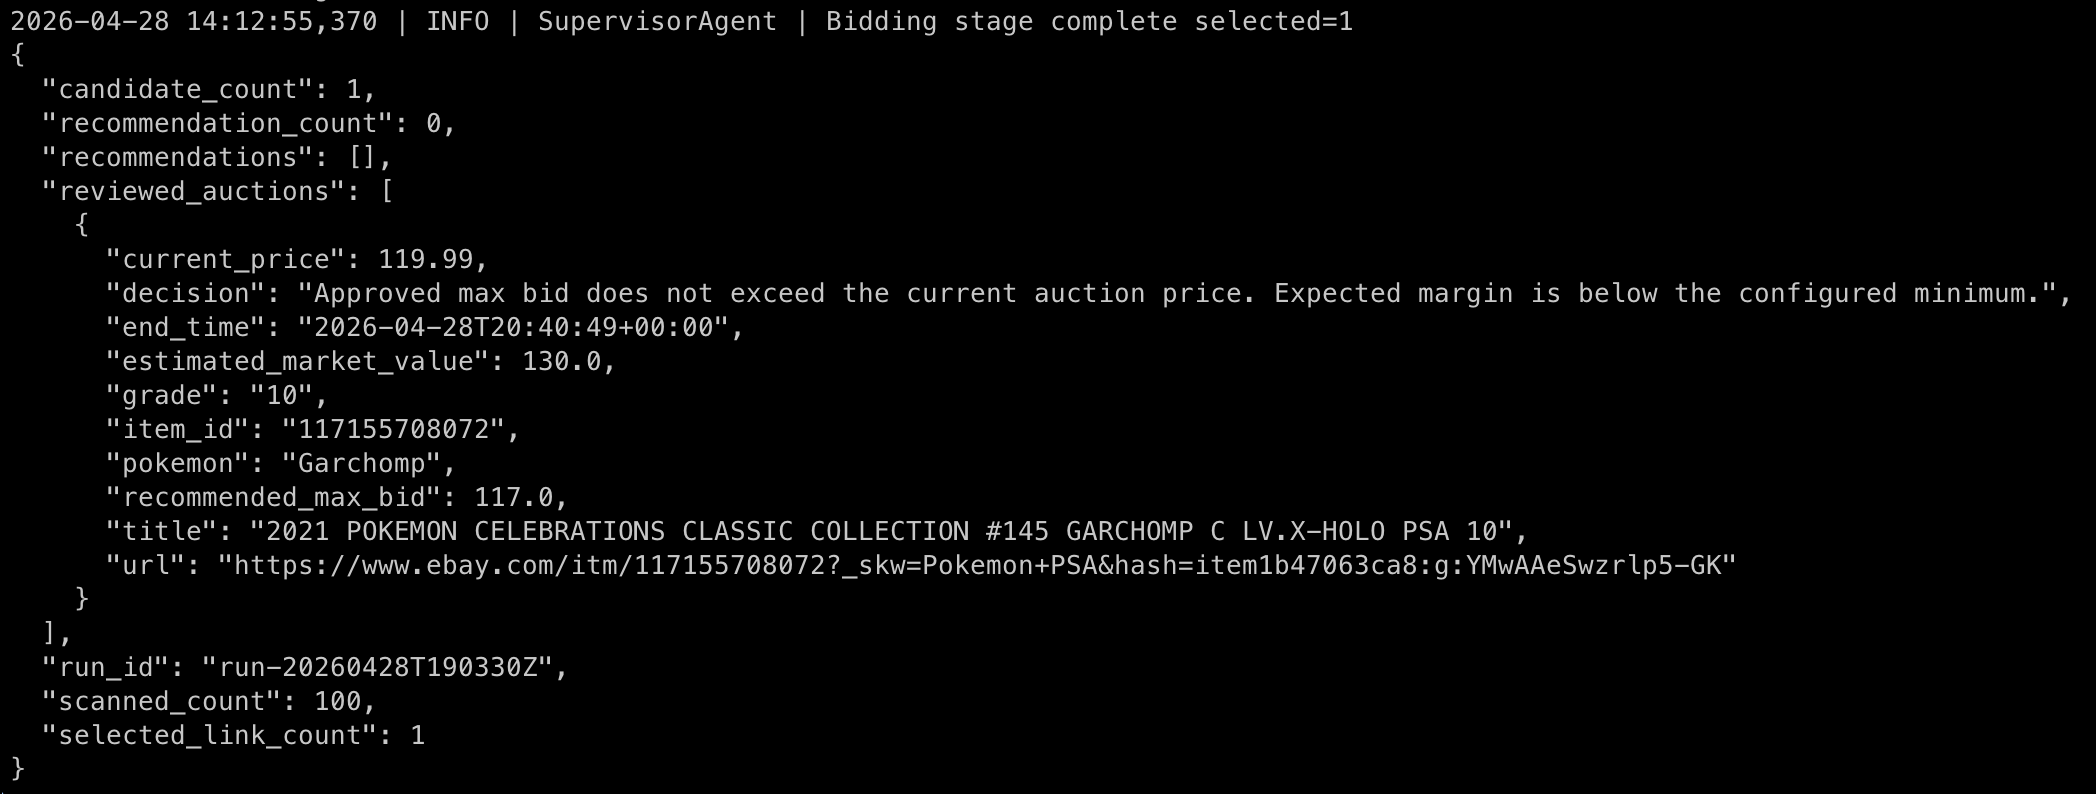
\includegraphics[width=.88\textwidth]{latex-final-images/early-garchomp-output.png}
    \caption{Early workflow output. The system scanned 100 listings, found one candidate, reviewed it, and denied it because the recommended max bid did not exceed the current auction price by enough to leave margin.}
    \label{fig:early-output}
\end{figure*}

\section{discovering}

The biggest thing I learned is that building an LLM application is less about asking one clever question and more about controlling the whole environment around the model. My first instinct was to let the LLM do the ``heavy lifting,'' but the project showed me that good agent systems need a partnership between flexible model reasoning and deterministic software boundaries.

The final system works in the sense that it can run locally, scan PSA auctions, process each auction one at a time, log each step, output denial or acceptance reasons, and produce manual bid recommendations only when the opportunity passes guardrails. It also works in dry-run mode with sample data and live mode when credentials are configured.

One concrete result was the per-auction workflow. Instead of collecting 100 listings, filtering them all, and then analyzing a batch later, the system now prints a clear beginning and ending for each listing:

\begin{verbatim}
------ Start auction 1/100 ------
Step 1: Checking listing requirements...
Step 2: Asking the listing-review agent...
Step 3: Researching market value...
Step 4: Asking the analysis agent...
Step 5: Applying bid safety rules...
Final decision: DENIED. Reason: ...
------ End auction 1/100: denied ------
\end{verbatim}

This made the project feel much more like an agentic review loop. It also made debugging easier because every listing has a stage, status, and reason.

Another result was learning how fragile marketplace valuation can be. For example, one early run found a Garchomp card and estimated its market value too high compared with manual eBay sold checks. Later, another Charizard example mixed low sold prices around \$27-\$30 with broad-search outliers above \$500. That produced an unsafe estimated value and an unsafe recommended bid before I improved the prompt and guardrails. Figure \ref{fig:outlier} shows the kind of output that revealed this problem.

\begin{figure*}[t]
    \centering
    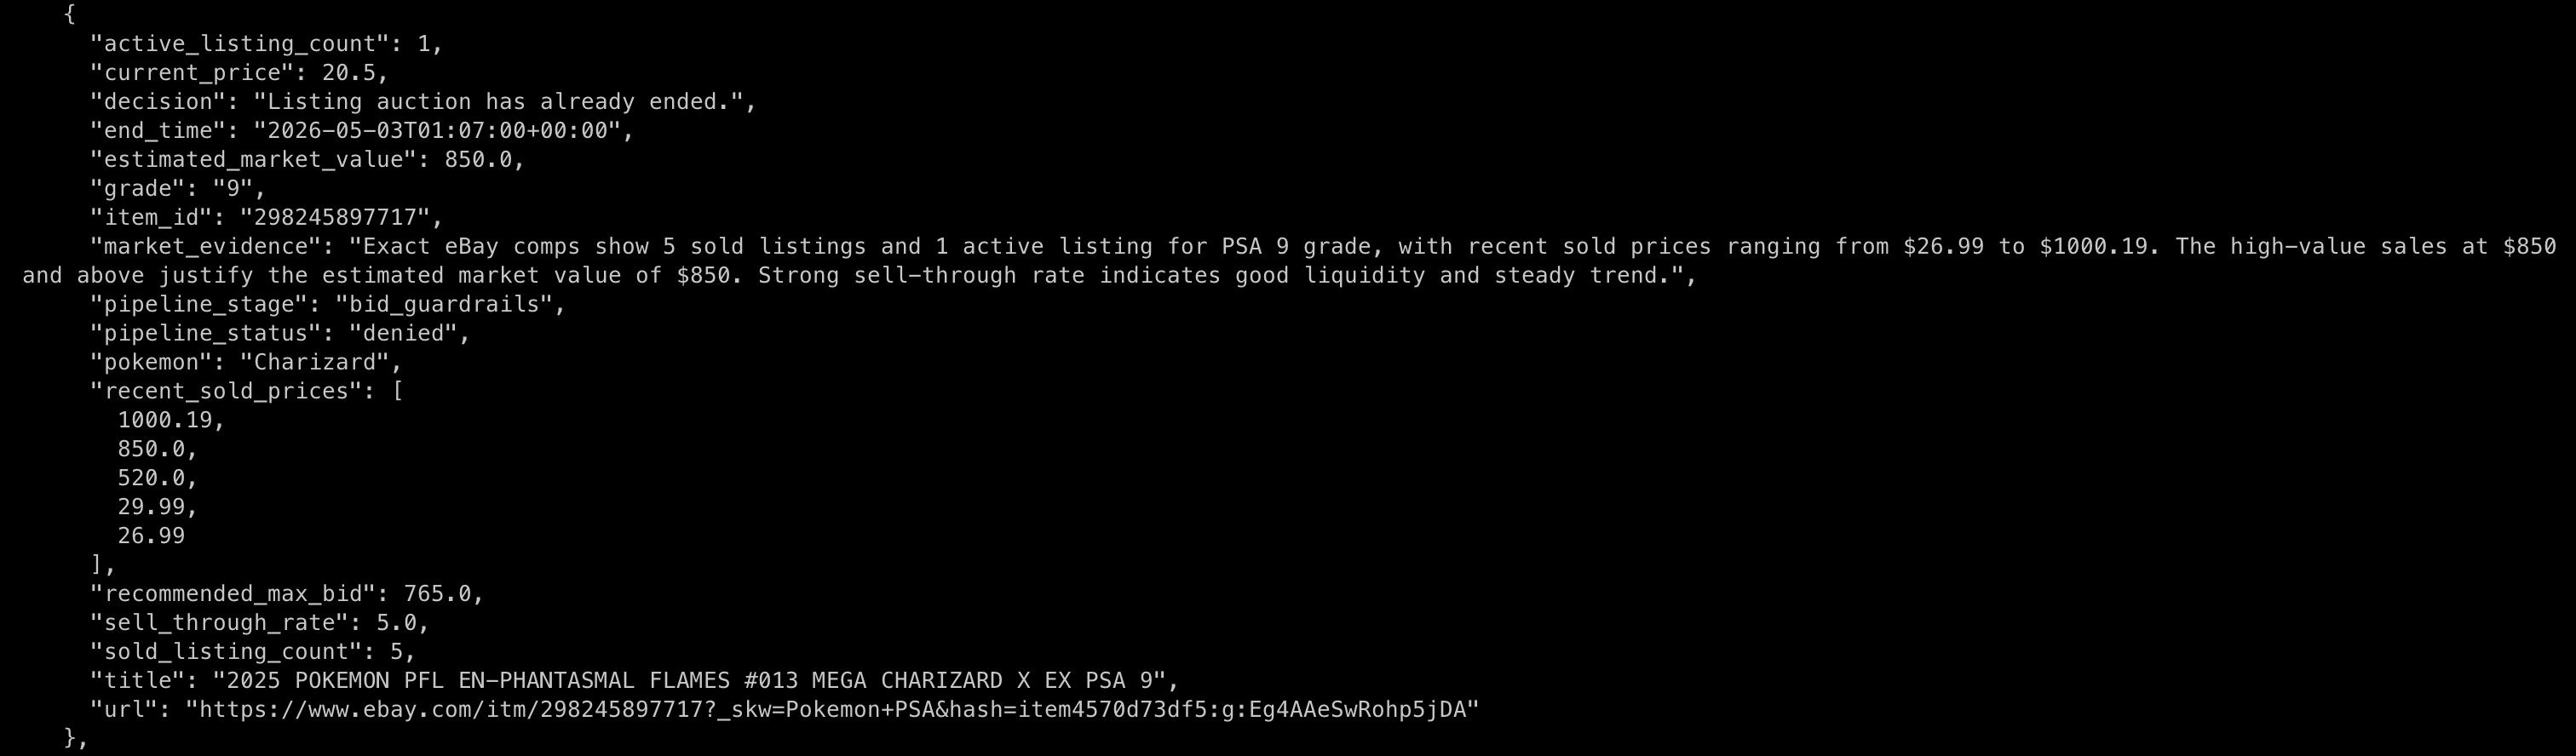
\includegraphics[width=.88\textwidth]{latex-final-images/outlier-charizard-output.png}
    \caption{A failure case that improved the project. The LLM saw incompatible sold-price clusters and over-valued the card. The final version now tells the market-research and analysis agents to reject unverified high-price clusters, and deterministic guardrails cap values using lower sold comps.}
    \label{fig:outlier}
\end{figure*}

The most important improvement was adding conservative valuation logic. If recent sold prices are spread out, the system now prefers the lower sold range or lower half of comps instead of the median or high end. For bidding, this matters because buying at the median can leave too little resale margin. A card selling between \$190 and \$250 should not automatically get a max bid around \$230. A safer system should often bid closer to 70--80\% of a conservative lower-comp value.

\begin{figure*}[t]
    \centering
    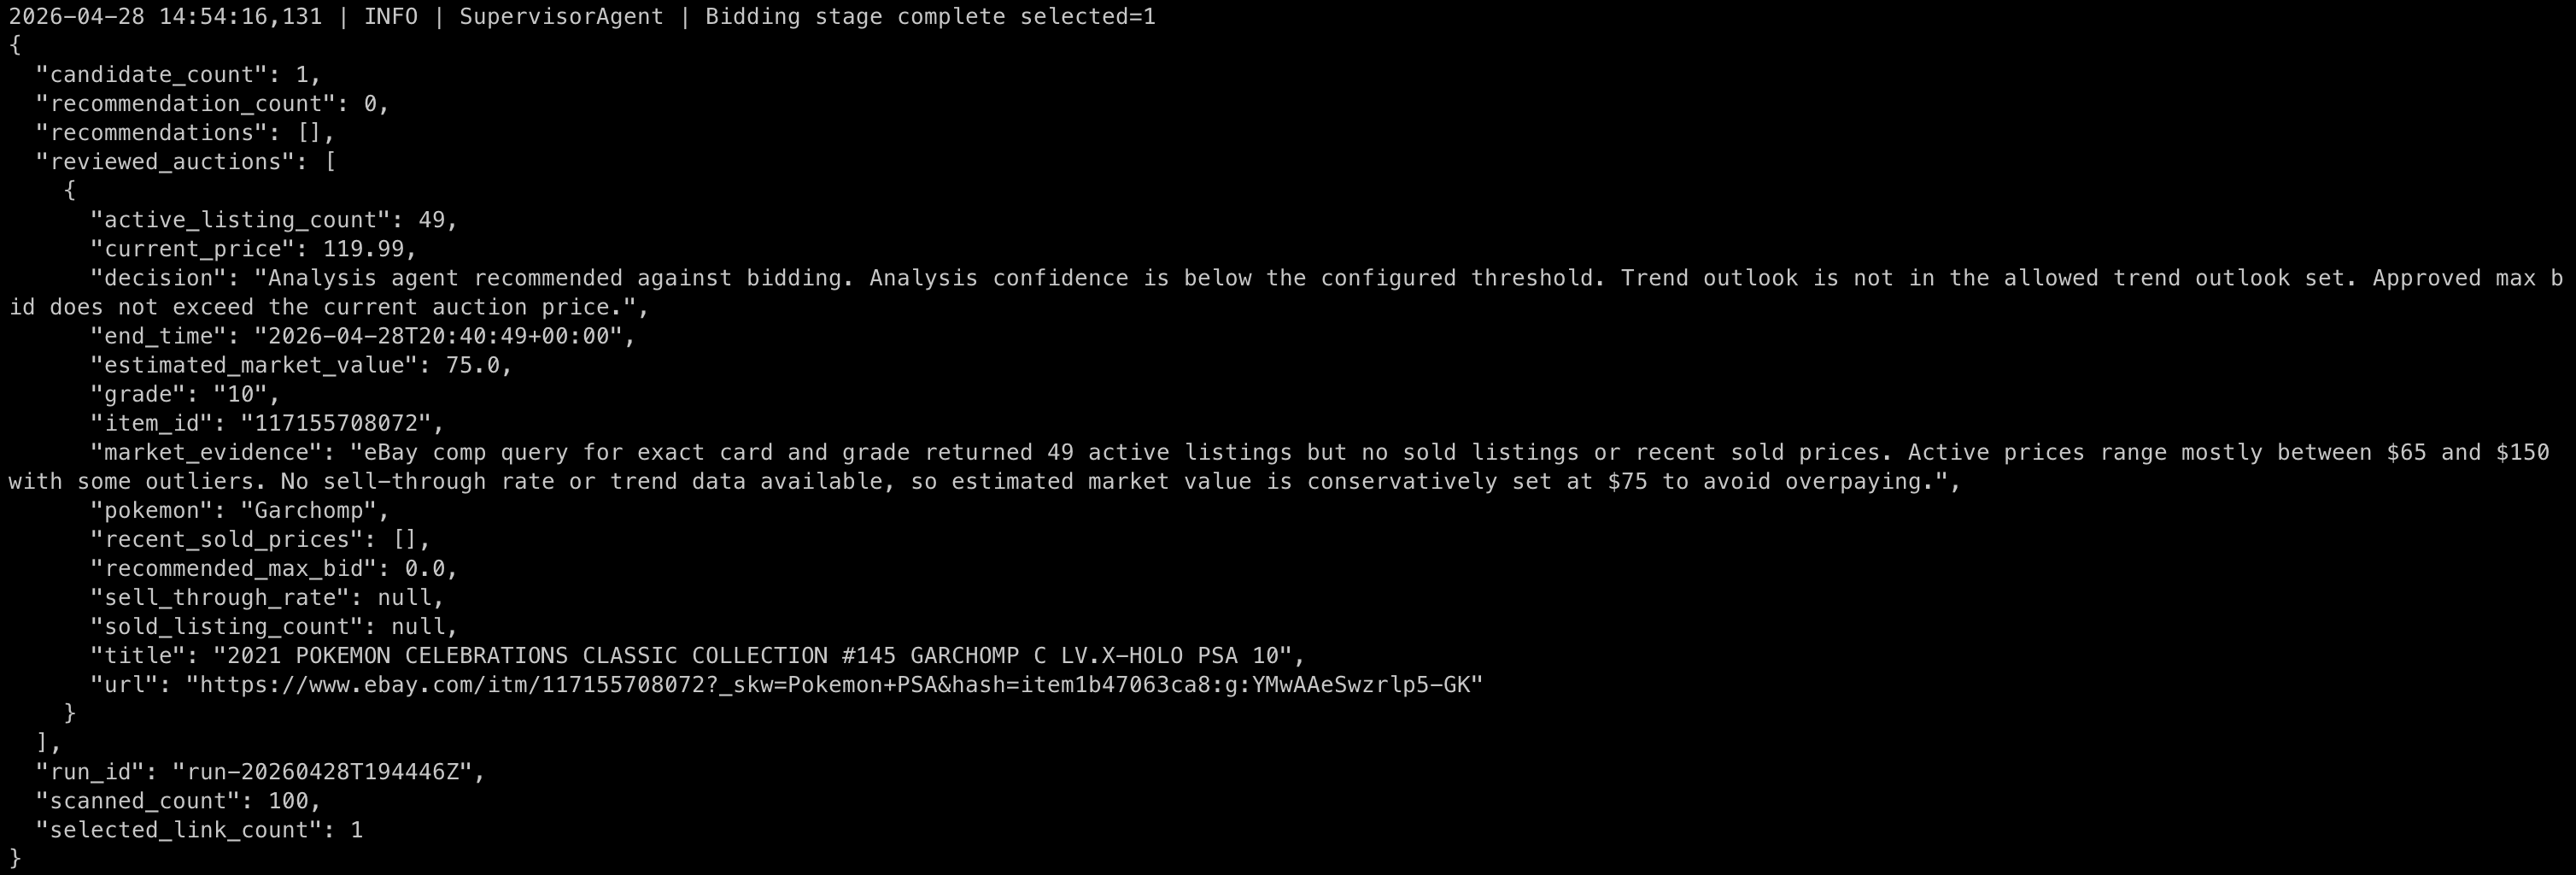
\includegraphics[width=.88\textwidth]{latex-final-images/garchomp-market-context-output.png}
    \caption{A later Garchomp review included market evidence fields such as active listing count, estimated market value, recent sold prices, sell-through rate, and a denial reason. This illustrates the move from free-form prose to structured evidence.}
    \label{fig:garchomp-context}
\end{figure*}

My self-assessment is that I started the class thinking mostly about LLMs as answer generators. This project moved me toward thinking about them as unreliable but powerful components inside larger systems. I now understand why agents need tools, schemas, logging, persistence, error handling, and guardrails. I also learned that ``LLM does the analysis'' does not mean ``Python trusts the LLM.'' The better design is to let the LLM reason about ambiguous market evidence, then make deterministic code check whether the result is safe enough to act on.

If I had more time, I would add a richer evaluation set of manually labeled listings. For each listing, I would record the true card identity, real sold comp range, correct market value, and whether a human card seller would bid. That would let me measure false positives and false negatives more rigorously. I would also improve market research by using a more reliable official sold-comps source if eBay grants access, because web-search evidence can still be incomplete or noisy.

\section{Class Topic 1: Prompt engineering}

This project illustrates prompt engineering because the behavior of the LLM agents changed dramatically as the prompts became more specific. At first, the analysis agent sometimes used active listing prices or broad-market guesses. That was not good enough for a bidding assistant. The final prompts tell the model exactly what role it has, what evidence counts, what evidence does not count, and what to do when information is missing.

I used three prompting techniques from class:

\begin{enumerate}[leftmargin=*]
    \item \textbf{Role/persona prompting}: the market-research agent acts like a professional trading-card comp analyst, and the analysis agent acts like a conservative PSA Pokemon card investment analyst and risk manager.
    \item \textbf{One-shot learning}: the prompt includes an example where sold comps contain \$25-\$30 prices mixed with \$500-\$1000 prices. The example teaches the model that this is probably a mismatch/outlier problem and should not produce a huge max bid.
    \item \textbf{Chain-of-thought style reasoning}: the prompt asks the model to reason internally step by step about identity, comps, outliers, liquidity, trend, and max bid. The final output does not reveal hidden chain-of-thought; it gives a concise evidence summary.
\end{enumerate}

For a beginning student, the lesson is that prompt engineering is not just ``ask nicely.'' It is a way of writing instructions that define the task, the role, the evidence standard, the output format, and examples of correct behavior.

\section{Class Topic 2: Agents and task decomposition}

This project illustrates agents because the system is broken into specialized roles. A scanner gets listings. A validation tool checks hard requirements. A listing-review agent decides if a candidate is worth researching. A market-research agent gathers comps. An analysis agent estimates value and max bid. A bid-execution tool applies final guardrails.

This is task decomposition: instead of one giant prompt doing everything, each step has a narrower responsibility. That matters because marketplace bidding has many failure points. If the parser incorrectly detects the Pokemon, the listing should fail before market research. If the market-research agent cannot find reliable sold comps, the analysis agent should not invent a value. If the analysis agent recommends a bid, the Python guardrails still check confidence, margin, max cap, seller, and auction status.

The supervisor coordinates the handoffs. In the final version, each listing moves through the full pipeline before the next listing starts. That made the workflow easier to understand and closer to how a human assistant might review auctions one by one.

\section{Class Topic 3: Tool use and external data}

The project illustrates tool use because the LLMs do not work from memory alone. They operate in a system that uses eBay data, listing-page enrichment, market-search evidence, and local storage. The eBay Browse API is used to search item summaries and retrieve auction listing details \cite{ebaybrowse}. The project also has a future official bidding adapter for eBay's proxy-bid endpoint, but that path requires a user token with the \texttt{buy.offer.auction} scope and eBay approval \cite{ebayproxybid}.

For a beginning student, a tool-using agent is an LLM that can interact with outside systems. In this project, the outside systems include:
\begin{enumerate}[leftmargin=*]
    \item eBay Browse API for active PSA auction data,
    \item web-search market research for sold comps and active comps,
    \item SQLite for persistence,
    \item deterministic Python parsers and validators, and
    \item manual eBay listing URLs for final user action.
\end{enumerate}

The important lesson is that the model alone is not the product. The product is the combination of model reasoning, external information, and safe software behavior.

\section{Class Topic 4: Structured output and typed models}

This project illustrates structured output because the agents do not return only paragraphs. They return objects such as \texttt{AnalysisResult} and \texttt{MarketResearchResult}. LangChain supports structured output so that agent responses can be captured in predictable schemas instead of being parsed from free text \cite{langchainstructured}. Pydantic helps define and validate those schemas \cite{pydanticjsonschema}.

This was important because the downstream code needs fields like:

\begin{verbatim}
should_bid: bool
confidence: float
estimated_market_value: float | None
recommended_max_bid: float | None
risk_flags: list[str]
\end{verbatim}

If the LLM only wrote prose, then the bid guardrails would need to scrape numbers out of text, which is brittle. With structured outputs, Python can directly check whether the confidence is too low, whether the max bid exceeds the cap, whether the margin is large enough, and whether the trend outlook is acceptable.

\section{Class Topic 5: Evaluation, guardrails, and human oversight}

This project illustrates evaluation and guardrails because correctness is not just whether the LLM sounds plausible. The system must avoid unsafe recommendations. A wrong bid can lose real money.

The final system includes several guardrails:
\begin{enumerate}[leftmargin=*]
    \item reject listings outside the target Pokemon allow-list,
    \item reject non-PSA or wrong-grade listings,
    \item reject missing or unreliable market evidence,
    \item reject low-confidence analysis,
    \item reject uncertain or downward trends,
    \item reject low expected margin,
    \item cap bids using a configured maximum budget,
    \item cap valuations toward lower sold comps when comps are spread out, and
    \item default to manual bidding, not automatic website bidding.
\end{enumerate}

Figure \ref{fig:high-value} shows another example of the structured review output. Even when the LLM finds high-value comps, the final system still checks whether the auction is active, whether the max bid is below current price, and whether the evidence supports a safe recommendation.

\begin{figure*}[t]
    \centering
    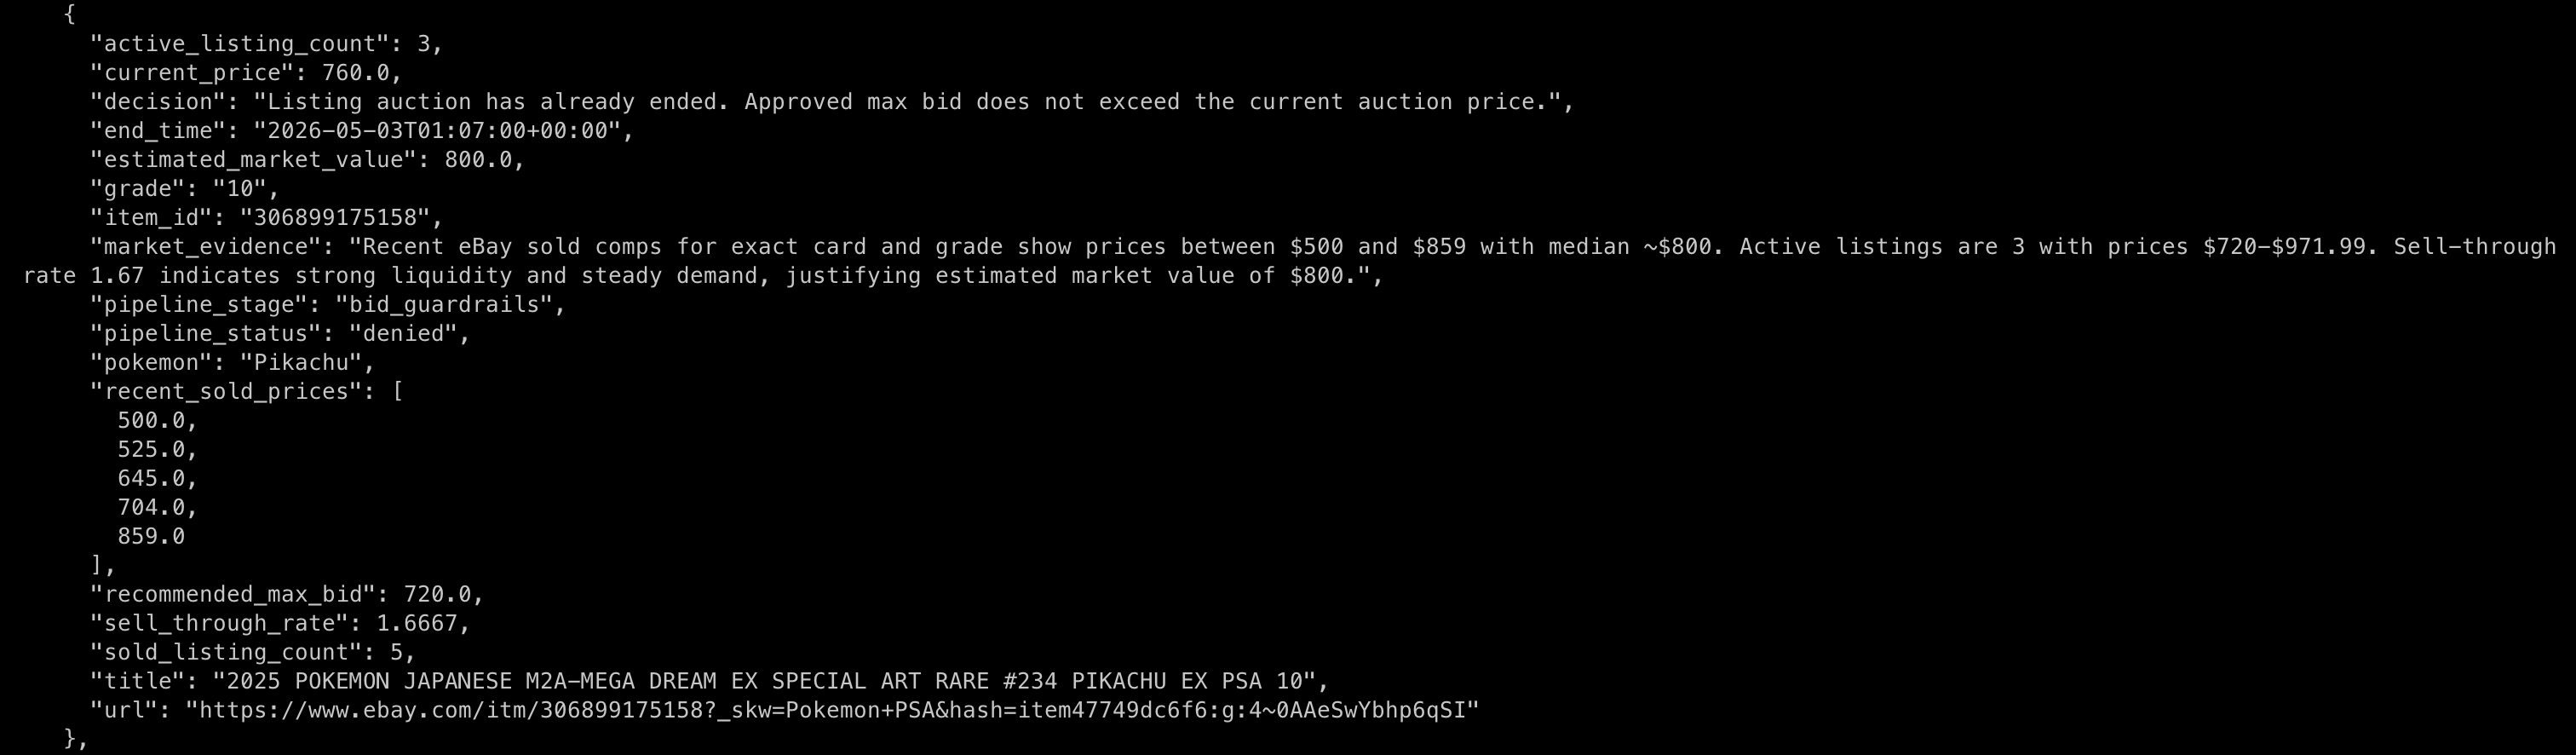
\includegraphics[width=.88\textwidth]{latex-final-images/high-value-pikachu-output.png}
    \caption{Structured review output for a high-value Pikachu listing. The output includes active count, sold prices, sell-through rate, estimated value, max bid, pipeline stage, and denial reason.}
    \label{fig:high-value}
\end{figure*}

The human oversight design also changed during the project. The original idea included automatic bidding. After researching eBay API constraints and thinking about platform safety, I changed the default MVP to manual bidding. The app can recommend a bid and open the listing URL, but the user must manually decide whether to bid. This keeps the project safer and more realistic.

\section{Correctness and completeness}

The code and resources are present in the shared project directory. The repository includes the Python source code, prompts, Pydantic models, tests, README, requirements file, sample data, SQLite storage code, OAuth helper script, and final writeup assets.

The implemented MVP works as claimed:
\begin{enumerate}[leftmargin=*]
    \item It can run locally in dry-run mode from sample data.
    \item It can use the official eBay Browse API when credentials are configured.
    \item It processes PSA auctions one listing at a time.
    \item It filters listings before deeper LLM analysis.
    \item It uses prompt-driven agents for listing review, market research, and max-bid analysis.
    \item It logs accepted/denied decisions and reasons.
    \item It produces actionable manual recommendations only after guardrails pass.
    \item It does not use Selenium, Playwright, cookie replay, copied browser requests, or website automation for bidding.
\end{enumerate}

The current automated test suite passes with 66 tests. These tests cover parsing, validation, prompt requirements, market-research handling, workflow output, OAuth helpers, bid guardrails, and safe bidding modes. I also manually inspected outputs such as the examples shown in the figures.

External sources are cited in the bibliography. The eBay API claims are based on eBay developer documentation, the LangChain structured-output claims are based on LangChain documentation, and the typed-model claims are based on Pydantic documentation.

\section{limitations}

The largest limitation is market-value accuracy. LLM web research can still return incomplete or noisy evidence. eBay sold results are messy because listings may differ by language, card number, variant, autograph status, slab company, grade, or title wording. The system now uses conservative prompts and deterministic lower-comp caps, but it can still be wrong if the upstream evidence is wrong.

A second limitation is that the system does not yet have a labeled evaluation dataset. I have examples from real runs, but I do not yet have hundreds of manually verified listings with ground-truth market values and human bid/no-bid labels. Without that, evaluation is mostly workflow testing plus manual inspection.

A third limitation is language handling. The system now detects English and Japanese from PSA-style title text and item specifics, but some listings may omit language or use ambiguous set abbreviations. Japanese cards can have different prices from English cards, so language must remain a hard matching field in future improvements.

A fourth limitation is API access. The project can scan with eBay's Browse API, but official proxy bidding requires special production approval and the correct OAuth scope \cite{ebayproxybid}. The MVP therefore defaults to manual bidding.

There are also ethical issues. In a small-company context, this tool could help a seller make faster and more consistent buying decisions. In a big-company context, similar tools could increase competition against ordinary collectors and make auctions feel less fair. In a school or government context, the larger ethical concern is automated decision-making with financial consequences. A model can sound confident while being wrong, so any system that affects money should log evidence, explain decisions, and keep humans responsible for final action. For that reason, I think manual bidding is the right MVP default.

\section{Sharing (Optional)}

I am willing to share this project with future classes as an example of a practical multi-agent LLM application, especially because it includes both successful parts and honest failure cases.

I have not shared the full project publicly online yet. If I publish it later, I would remove secrets, document the eBay API constraints carefully, and make clear that browser automation bidding is intentionally unsupported.

\begin{thebibliography}{9}

\bibitem{handsonllm}
Jay Alammar and Maarten Grootendorst.
\textit{Hands-On Large Language Models}. Official code repository.
\url{https://github.com/HandsOnLLM/Hands-On-Large-Language-Models}

\bibitem{langchainstructured}
LangChain.
Structured output documentation.
\url{https://docs.langchain.com/oss/python/langchain/structured-output}

\bibitem{openaistructured}
OpenAI.
Structured outputs documentation.
\url{https://platform.openai.com/docs/guides/structured-outputs}

\bibitem{ebaybrowse}
eBay Developers Program.
Browse API item summary search documentation.
\url{https://developer.ebay.com/api-docs/buy/browse/resources/item_summary/methods/search}

\bibitem{ebayproxybid}
eBay Developers Program.
Buy Offer API \texttt{placeProxyBid} documentation.
\url{https://developer.ebay.com/api-docs/buy/offer/resources/bidding/methods/placeProxyBid}

\bibitem{pydanticjsonschema}
Pydantic.
JSON schema documentation.
\url{https://docs.pydantic.dev/latest/concepts/json_schema/}

\end{thebibliography}

\end{document}
